\part{Felhasználói dokumentáció}
A programcsomag JAVA programozási nyelven lett megvalósítva, ezért a program számára biztosítani kell JAVA futtatókörnyezetet, továbbá a program működéséhez adatbázisszerverre is szükség lesz. A telepítés magába foglalja az adatbázisséma elkészítését és az adatbázis rekonstrukciós célú adatokkal való feltöltését is, így a telepítést követően extra dolgokra nem lesz szükség a szoftver használatához. A telepítés közben a számítógépet újraindítani nem szükséges. A kiegészítő programcsomagok telepítési sorrendje nem lényeges.

\section{Követelmények}
A programcsomag használatához az alábbi rendszerkövetelményeknek teljesülniük kell, ellenkező esetben a program hibásan működhet.

\subsection{Hardver}
Az alábbi hardveres követelmények nem szigorúan értendők. Adott esetben gyengébb konfigurációjú számítógépen is elfuthat a programcsomag.
\begin{itemize}
\item Legalább Intel® Pentium® 4 Processor 2.80 GHz
\item Legalább 1GB RAM
\item Legalább 50MB szabad lemezterület
\end{itemize}

\subsection{Szoftver}
Az alábbi szoftveres követelmények szigorúan értendők. Az alacsonyabb verziószámú kiegészítő szoftvercsomagok nem megfelelők a programcsomag futtatásához. A magasabb verziószámmal ellátot kiegészítő szoftvercsomagok visszamenőleges kompatibilitásáról a mindenkori gyártó honlapján található információ.
\begin{itemize}
\item Legalább Windows XP operációs rendszer
\item Java SE Runtime Environment 8
\item MySQL Community Server 5.6
\end{itemize}

\section{Telepítés}
A telepítési leírás útmutató jellegű, rendszerkénti eltérés megfigyelhető. Az útmutató nem tér ki a telepítési folyamat minden lehetséges eshetőségére. Esetleges hibák esetén érdemes felkeresni a mindenkori szoftvercsomag interneten elérhető dokumentációját.

\subsection{Java SE Runtime Environment 8}
A programcsomag futtatásához legalább Windows XP operációs rendszer szükséges, amelyen Java SE Runtime Environment 8 futtató környezet \footnote{a továbbiakban JRE} \cite{jresite} fut. A JRE feltelepítését követően manuálisan ellenőrizzük, hogy a rendszer felvette-e környezeti változóként az installációs könyvtárat. Navigáljunk az operációs rendszerben a környezeti változók módosítása panelhez, majd ellenőrizzük le, hogy a PATH nevű környezeti változóhoz hozzá lett-e adva az installációs könyvtár, mint például: \path{C:\Program Files\Java\jre1.8.0_66\bin}. A telepítési könyvtár operációs rendszerenként eltérhet.

\begin{figure}[h!]
  \caption{PATH környezeti változó értéke}
  \label{fig:path_env}
  \centering
    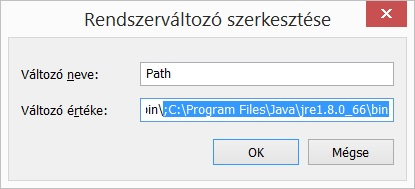
\includegraphics{user-documentation/images/path_env.jpg}
\end{figure}

Ha a JRE installációs könyvtár gyökerében található bin könyvtár nincs behivatkozva a PATH nevű környezeti változó értékéhez, akkor az \ref{fig:path_env}. ábrán látható módon egészítsük ki az értéket, majd mentsük el a változtatásokat és indítsuk el az operációs rendszer által szolgáltatott parancssort és ha sikeresen jártunk el, akkor a

\begin{Verbatim}[xleftmargin=.5in]
java -version
\end{Verbatim}
utasítás hatására a \ref{fig:jre_version}. ábrán látható szöveg jelenik meg a parancssoron, akkor sikeres volt a JRE telepítése és beállítása.
\begin{figure}[h!]
  \caption{JRE verzió}
  \label{fig:jre_version}
  \centering
    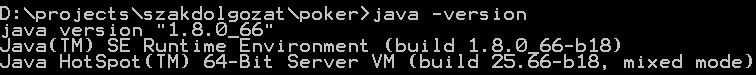
\includegraphics[width=14cm]{user-documentation/images/java_version.jpg}
\end{figure}
 
 \subsection{MySQL Community Server 5.6}
 A programcsomag megköveteli a MySQL Community Server 5.6 \footnote{a továbbiakban MySQL szerver} \cite{mysqlsite} adatbázis-kezelő rendszer használatát is. Letöltés után csomagoljuk ki a zip állományt egy tetszőleges könyvtárba, majd az előbiekkel megegyező módon adjuk hozzá a PATH nevű környezeti változó értékéhez a MySQL Server \texttt{bin} könyvtár elérési útvonalát. Ha a parancssor nyitva van, akkor zárjuk be és indítsuk el újra, majd navigáljunk a MySQL Server \texttt{bin} könyvtárába, ott pedig adjuk ki a
 \begin{Verbatim}[xleftmargin=.5in]
mysqld --install
\end{Verbatim}
parancsot. A parancs végrehajtása után navigáljunk a szolgáltatások panelhez, amelyet legkönnyebben a parancssorban a
 \begin{Verbatim}[xleftmargin=.5in]
services.msc
\end{Verbatim}
kiadott utasítással lehet elérni. Majd járjunk el a \ref{fig:mysql_service}. ábrának megfelelően. 

\begin{figure}[h!]
  \caption{MySQL Service}
  \label{fig:mysql_service}
  \centering
    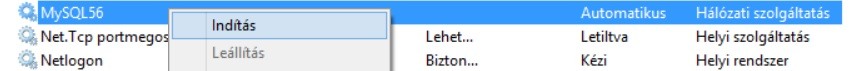
\includegraphics{user-documentation/images/mysql_service.jpg}
\end{figure}
Térjünk vissza a parancssorra, ahol adjuk ki a 
 \begin{Verbatim}[xleftmargin=.5in]
mysql -u root -p
\end{Verbatim}
parancsot, amely jelszót fog kérni. A beviteli sort hagyjuk üresen, nyomjunk entert. Ha sikeresen beléptünk az adatbázis-kezelő rendszerbe, akkor adjuk ki a
 \begin{Verbatim}[xleftmargin=.5in]
SELECT VERSION();
\end{Verbatim}
utasítást, és ha a \ref{fig:mysql_version}. ábrának megfelelő képernyőképet kapunk, akkor sikeresen feltelepítettük az adatbázis-kezelő rendszert.
\begin{figure}[h!]
  \caption{MySQL Server verzió}
  \label{fig:mysql_version}
  \centering
    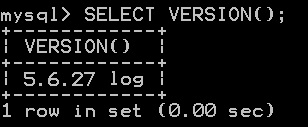
\includegraphics{user-documentation/images/mysql_version.jpg}
\end{figure}

\subsection{Az adatbázis használatba vétele}
Ha sikeresen elindítottuk a MySQL Servert, akkor szükségünk lesz egy új adatbázissémára és demóadatokra, amelyet a \path{X:\poker\release\poker-db.sql} állományban találunk. Az \path{X} kötetcímke jelöli jelenleg és a későbbiek során is a DVD meghajtót, amelybe a DVD lemezt helyeztük. Ezt a fájlt kell lefuttatni az adatbázis szerveren. Egymás után többszöri futtatás esetén is ugyanazt az eredményt kapjuk. Az adatbázis-kezelő rendszerből lépjünk ki a 
\begin{Verbatim}[xleftmargin=.5in]
quit
\end{Verbatim}
paranccsal, majd a parancssorban adjuk ki a
 \begin{Verbatim}[xleftmargin=.5in]
mysql -u root -p < X:\poker\release\poker-db.sql
\end{Verbatim}
utasítást. A parancs kiadását követően az adatbázis-kezelő rendszer jelszót fog kérni. A beviteli sort ugyancsak hagyjuk üresen. Ha sikeresen lefutott a parancs, akkor az adatbázisséma elkészült és a program demóadatokkal is feltöltötte.

\section{Fogalomtár}
A játékhoz feltétlenül szükséges fogalmak, amelyeket a dokumentáció későbbi fejezetei felhasználnak.
\subsection{Parancsok}
Az alábbi parancsokat a felhasználók tudják kiadni. A szerver biztosítja, hogy csak a megfelelő parancsok legyenek hívhatóak a póker partik során.
\pokerparagraph{CALL}
A felhasználó ezt a parancsot adja ki, ha a tartozását ki szeretné egyenlíteni az asztal felé.
\pokerparagraph{CHECK}
Játékos által kiadható parancs, melyet akkor kell kiadnia, amikor a játékos nem tartozik az asztal felé, és emelni sem szeretné a tétet.
\pokerparagraph{BLIND}
Olyan parancs, amelyet a kliens oldali program automatikusan hív meg. Ha a szerver \texttt{BLIND} típusú utasítást küld, akkor a kliens automatikusan beteszi a kis vagy nagy vakot az asztalra attól függően, hogy a szerver mire kötelezte az adott felhasználót. A kis vak, vagy angol nevén \texttt{small blind} az asztalnál érvényben lévő alaptét felét, míg a nagy vak, vagy angolul big \texttt{blind} az asztalra vonatkozó alaptét egészét jelenti.
\pokerparagraph{RAISE}
Olyan speciális parancs, amely hatására a felhasználó tartozása kiegyenlítésre kerül az asztal felé és még emel a téten az asztal alaptétjének megfelelő értékkel.
\pokerparagraph{QUIT}
Asztal elhagyására szolgáló parancs. A kilépését követően a program visszairányítja a felhasználót a táblalistázó oldalra. Ha bármilyen oknál fogva a gomb letiltásra kerül és a játékos nem tudja elhagyni az asztalt, ez esetben a billentyűzeten a \texttt{Q} gombot megnyomva visszakerül a játékos a táblalistázó felületre. Fontos megjegyezni, hogy a gomb a póker partik közben csak akkor van engedélyezve, ha éppen az adott felhasználó következik. Ha az asztal megfelelően működik és a játékos mégis úgy dönt, hogy ezt a funkciót kihasználva hagyja el a játékasztalt, akkor a gondolkodási idő lejárta után az asztal eltávolítja a játékost az asztaltól és a parti folytatódik tovább. A kliensnél ekkor a táblalistázó felület töltődik be.
\pokerparagraph{CHANGE}
A parancs csak a classic játékstílusban érhető el. A parancs meghívásával a felhasználó utasítja a programot, hogy a cserére megjelölt kártyalapokat a szerver új kártyalapokkal helyettesítse. Az új kártyalapok csak akkor kerülnek kiosztásra, ha minden játékos nyilatkozott az adott körben.
\pokerparagraph{LOG}
A felhasználó játék közben korlátozott mértékben vissza tudja nézni a már megtörtént főbb eseményeket. Például az előző játékos milyen parancsot hajtott végre.
\subsection{Fogalmak}

\pokerparagraph{FLOP}
Texas Hold'Em játékstílusú játékban a szerver kiosztja az első három közös lapot.
\pokerparagraph{TURN}
Texas Hold'Em játékstílusú játékban a szerver kiosztja a negyedik közös lapot.
\pokerparagraph{RIVER}
Texas Hold'Em játékstílusú játékban a szerver kiosztja az ötödik közös lapot.
\pokerparagraph{Dealer}
Magyarul osztó. A játék során az osztógomb, amely a grafikus felületen \texttt{D} betűvel van jelezve. Az óramutató járásával megegyező irányban halad körbe az asztalon, így minden parti esetén más felhasználó tölti be az a osztó szerepét.

\section{A póker játékról}
A póker \cite{poker_game}, mint kártyajáték igen népszerű szerencsejáték. Akár élő tv adásokat is végig lehet követni, ahol hatalmas főnyereményeket osztanak ki a dobogós helyezetteknek. Viszonylag sokfajtája terjedt el szerte a világon, kezdve a klasszikus 5 lapos leosztásokkal egészen az OMAHA játékstíluson át a jól ismert Texas Hold'Em játékstílusig. A játékot 52 lapos francia kártyapaklival játszák, amelyben 4 szín és 13 különböző értékű kártyalap található. A játékstílusok igen különbözőek tudnak lenni. Megkölönböztetünk \texttt{ante}, illetve \texttt{blind} alaptétet. \texttt{Ante} alaptét esetén az asztalnál ülő összes játékos előre meghatározott tétet rak be. \texttt{Blind} alaptét esetén megkülönböztetünk kis és nagy vakot, amelyet körönként más és más játékosok raknak be. Minden esetben az osztótól közvetlenül balra ülő játékosnak kell beraknia a kis vakot. Az osztótól kettővel balra ülő játékosnak pedig a nagy vakot. Amíg az alaptétek nem kerültek be az asztalra, addig a ház nem kezdi meg a lapok kiosztását. \\
A \ref{fig:omaha}. ábrán látható az OMAHA \cite{omaha_poker} játékstílus. A Texas Hold'Em játékstílushoz igen hasonló pókerjáték változat. A játékosok a kezükbe négy darab kártyalapot kapnak a vakok betétele után, majd megkezdődik az első licitkör, amelynek a végén három közös lap kerül ki az asztal közepére. Újabb licitkör kezdődik, amelynek a végén egy, majd az újabb licitkör végén, még egy újabb kártyalap kerül az asztal közepére, mint közöslap. A felhasználóknak maximum öt lapot lehet felhasználniuk a legjobb kéz előállítására. Az öt lapból kötelezően kettő a saját kézből történik a maradék három pedig a közös lapokból. Értelemszerűen a legerősebb kéz nyer \cite{card_combinations}. A játék célja, hogy minél több zsetont gyűjtsünk össze a partik során.
\begin{figure}[h!]
  \caption{OMAHA póker játék}
  \label{fig:omaha}
  \centering
    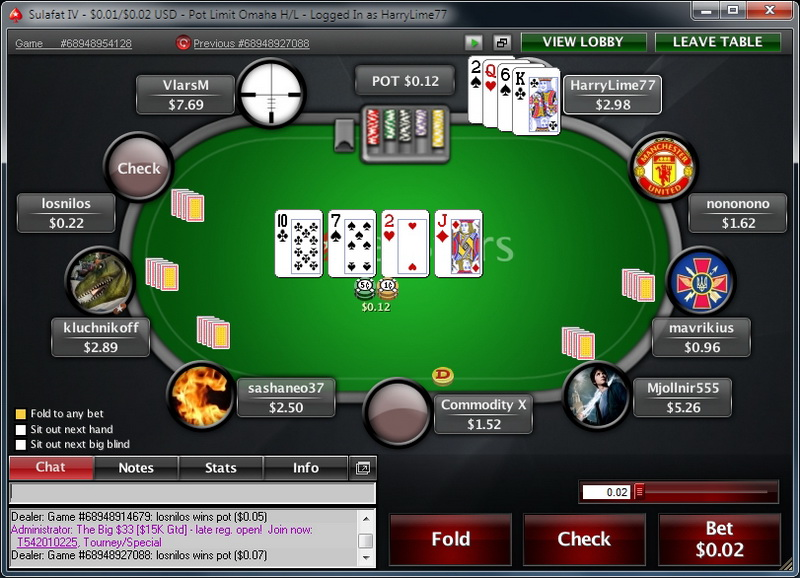
\includegraphics[width=\textwidth]{user-documentation/images/omaha.jpg}
\end{figure}

\subsection{Játékmenet}
Minden játékszerver úgy lett konfigurálva, hogy két játékos esetén a parti elkezdődjön. Ha valaki később csatlakozott az asztalhoz, az a megkezdett partiból semmit nem érzékel, mintha üres asztalnál ülne. Csak a következő partiba tud beszállni. Mindkét játékstílus esetén van egy \texttt{BLIND} kör, amikor a szerver bekéri a vakokat a játékosoktól. Az osztótól eggyel balra ülő játékos köteles betenni a kis vakot, a kis vaktól eggyel balra ülő játékos pedig köteles betenni a nagy vakot. Ebból a felhasználó nem lát semmit, egy automatizált eljárás hajtja végre a vakok beadását. Az osztógomb  a legelső körben kerül kiosztásra a legelsőként csatlakozott játékoshoz. Az osztógomb az óramutató járásával megegyező irányban halad. Minden új megkezdett parti esetén az osztógomb a következő játékoshoz kerül. Minden parti legelső körében a kezdő játékos az osztótól balra ülő harmadik játékos, minden további kört a kis vakra kötelezett játékos kezd meg.  \\
A játékszerverek nem képesek kezelni, ha egy játékosnak elfogyott, illetve nincs elegendő zsetonja. Ebből kifolyólag esetenként előfordulhat negatív egyenleg, illetve nem definiált viselkedés. A játékosok szigorúan csak egymást követve küldhetnek utasításokat a szervernek. A felhasználói grafikus felületen egyértelmű jelzéssel van ellátva az éppen soron levő játékos. A játékosok megadhatják, emelhetik a tétet, illetve, ha nem szeretnének az adott körben semmit csinálni, akkor CHECK típusú üzenetet is küldhetnek a szervernek. Az emelés mértéke a mindenkori játékasztal alaptét felét jelenti. Ugyanakkor lap eldobásra és a játék elhagyására is lehetőség van. A felhasználók korlátozottan visszanézhetik a korábbi leosztásokat, és a partiban történt eseményeket. A játékosok asztalonkénti maximum száma 5 fő. A kliensek a játék elhagyását követően újracsatlakozhatnak az adott játékszerverre a fentieket figyelembe véve. Lehetőség van asztalt váltani, és a játékszerverek korlátozottan képesek kezelni, ha a játékossal megszakad a kapcsolat. A kliens alkalmazások is korlátozott mértékben fel vannak készítve az esetleg kommunikációs hibákra.

\clearpage

\subsection{Játékstílusok} \label{subsubsec:game_styles}
A póker játék meglehetősen sok játékstílusban terjedt el szerte a világon. Régebben még a kártyapakli is eltért a ma használatos 52 lapos francia kártyapaklitól. A játékstílusok közül kettőt valósít meg a programcsomag
\begin{itemize}[leftmargin=2cm]
\item Classic \cite{five_card_draw}
\item Texas Hold'Em \cite{texas_holdem}
\end{itemize}
A két játékstílus közötti legfőbb különbség, hogy a klasszikus játékstílus esetén nincsenek közös lapok, míg Texas Hold'Em játékstílus esetén vannak.

\pokerparagraph{Classic} 
A klasszikus játékstílus legfőbb ismertető jele, hogy mindenki öt lapot kap kézbe és nincsenek közös lapok. Először is a vakokra kötelezett játékosok automatizált formában rakják be a vakokat, azután pedig úgynevezett előkör van, amikor a szerver minden játékosnak 5-5 darab kártyalapot oszt kézbe és ezek alapján lehet licitálni. Ha vége a körnek, akkor mindenki kicserélheti a lapjait, amiket saját maga választ ki a grafikus felületen a saját kártyalapjainak rákattintásával. Ha a kártyalap feljebb csúszott a grafikus megjelenítésen, akkor a kártyalapot cserére jelölte a játékos. A \texttt{Change} feliratú gombbal cserélhetők a kártyák. Mindenki akkor kapja meg az új kártyalapjait, ha már mindenki nyilatkozott a cseréről. Ezek után új kör indul, amikor is az új lapok birtokában tehetik meg a tétjeiket a játékosok. A kör után a szerver kihirdeti a nyertest, és a nyertes lapokat az asztal közepén jeleníti meg a grafikus felület. Kivétel, ha az éppen adott felhasználó a nyertes, akkor a nyertes kártyalapok maga előtt jelennek meg, iyenkor más kártyalapok nem kerülnek felfordításra. A felhasználók a nyertes lapok megtekintését követően kötelesek rákattintani a \texttt{Check} feliratú gombra, illetőleg ha kifutnak az időből, akkor a játék asztal kilépteti őket. Ha ebben a körben is mindenki nyilatkozott, akkor a játékasztal új partit indít.

\pokerparagraph{Texas Hold'Em}
A klasszikus játékstílussal erősen megegyező játékmenetű stílus. A különbség csupán annyi, hogy a szerver, ami a ház szerepét tölti be, 2-2 darab kártyalapot oszt minden játékosnak a kezébe, amelyekkel a játékosok a parti végéig rendelkeznek. Illetőleg a nyertes lapok semmilyen esetben sem középen, hanem a játékosoknál jelennek meg.

\section{Futtatás}

\subsection{A póker szerver indítása}
Az \path{X:\poker\release} nevű mappában található meg  a poker-server-1.0.0.jar fájl. Nyissunk egy terminált a kijelölt könyvtárban, és adjuk ki a
 \begin{Verbatim}[xleftmargin=.5in]
java -jar poker-server-1.0.0.jar
\end{Verbatim}
parancsot. Ha a \ref{fig:server_started}. ábrának megfelelő parancssori naplózást látunk, akkor a szervert sikeresen elindítottuk.
\begin{figure}[h!]
  \caption{Szerver naplózása}
  \label{fig:server_started}
  \centering
    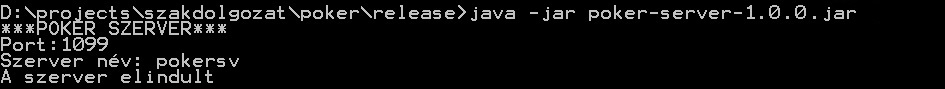
\includegraphics[width=\linewidth]{user-documentation/images/server_started.jpg}
\end{figure}

\subsection{A póker kliens indítása}
A kliens futtatása hasonló módon történik, mint a szerveré. Navigáljunk a \path{X:\poker\release} mappába, és a parancssorban adjuk ki a megfeleő parancsot. Ha a kliens sikeresen elindult, akkor a \ref{fig:server_search}. ábrának megfelelő képernyőképet kapunk. Ha a szervert lokálisan indítottuk, akkor a beállításokat ne módosítsuk. A sikeres csatlakozást követően a program egy bejelentkező felületre irányítja a felhasználót. \\

\begin{figure}[h!]
  \caption{Szerver keresés}
  \label{fig:server_search}
  \centering
    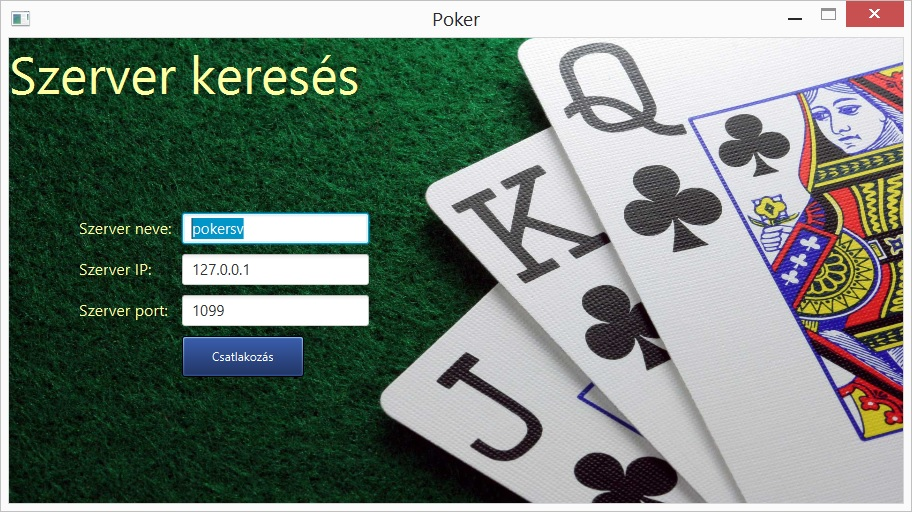
\includegraphics[width=\linewidth]{user-documentation/images/server-search.jpg}
\end{figure}

\section{A póker játék használata}

Ha még nem regisztráltuk magunkat a játékba, akkor kattintsunk a \texttt{Regisztráció} nevű gombra. Adjuk meg a regisztrálni kívánt felhasználó nevünket és jelszavunkat, majd regisztráljunk. A szerver értesít minket, hogy a művelet sikeres, vagy sikertelen volt. A \ref{fig:reg_succ}. ábra egy sikeres regisztrációt szemléltet. Azonban ha játékadminisztrátorként szeretnénk belépni a játékba, azt az \texttt{admin/admin} felhaszálónév-jelszó párossal tehetjük meg. Továbbá vannak előre definiált játékosok is, amelyekhez a \texttt{test} jelszóval tudunk belépni. A felhasználónevek pedig \texttt{test1}, \texttt{test2}, \texttt{test3} és \texttt{test4}.
\begin{figure}[h!]
  \caption{Sikeres regisztráció}
  \label{fig:reg_succ}
  \centering
    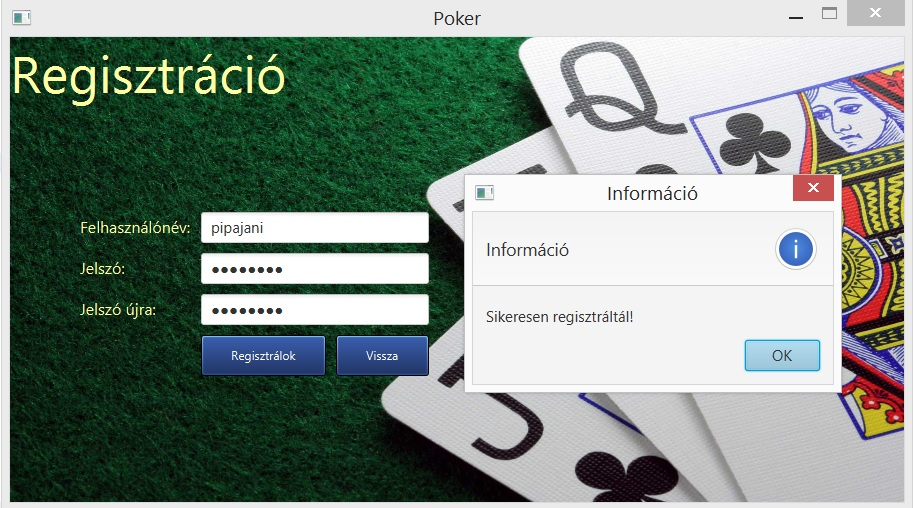
\includegraphics[width=\linewidth]{user-documentation/images/succ_reg.jpg}
\end{figure}
Ügyeljünk arra, hogy névütközéseket a szerver nem enged. Tehát, ha valaki \texttt{XYZ} névvel már regisztrálva van, akkor még egy ugyanolyan nevű felhasználót nem enged regisztrálni a szerver. Továbbá győződjünk meg arról, hogy a megadott jelszavak megegyeznek.  \\
Sikeres regisztrációt követően a program visszairányít minket a bejelentkezési formhoz, amelyet értelemszerűen kitöltve be tudunk jelentkezni a programba.
A sikeres bejelentkezést követően a \ref{fig:poker_tables}. ábrán látható felület fogad minket, ahol például asztalhoz csatlakozhatunk. Tetszőlegesen válasszunk ki egy Texas Hold'Em játékstílusú asztalt, majd kattintsunk a \texttt{Csatlakozás} feliratú gombra.
\begin{figure}[h!]
  \caption{Játékasztalok}
  \label{fig:poker_tables}
  \centering
    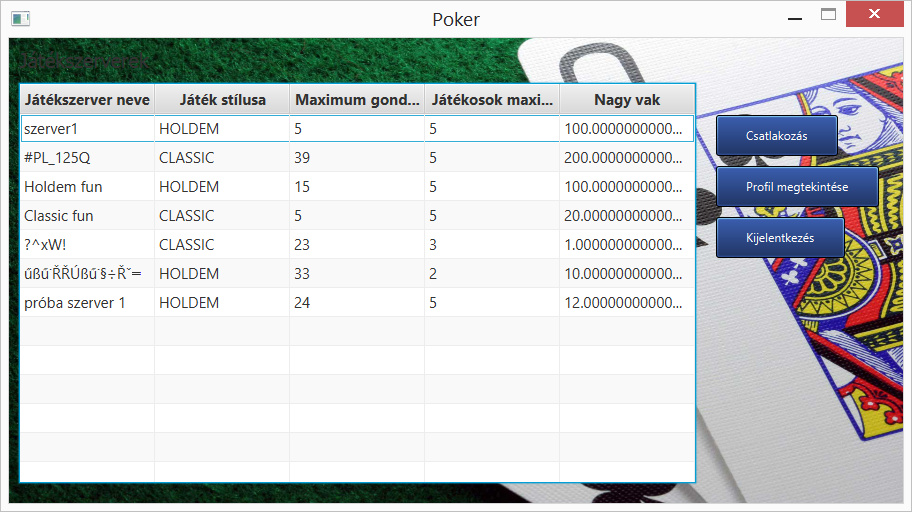
\includegraphics[width=\linewidth]{user-documentation/images/tables.jpg}
\end{figure}

\begin{figure}[h!]
  \caption{Üres játékasztal}
  \label{fig:parti_1}
  \centering
    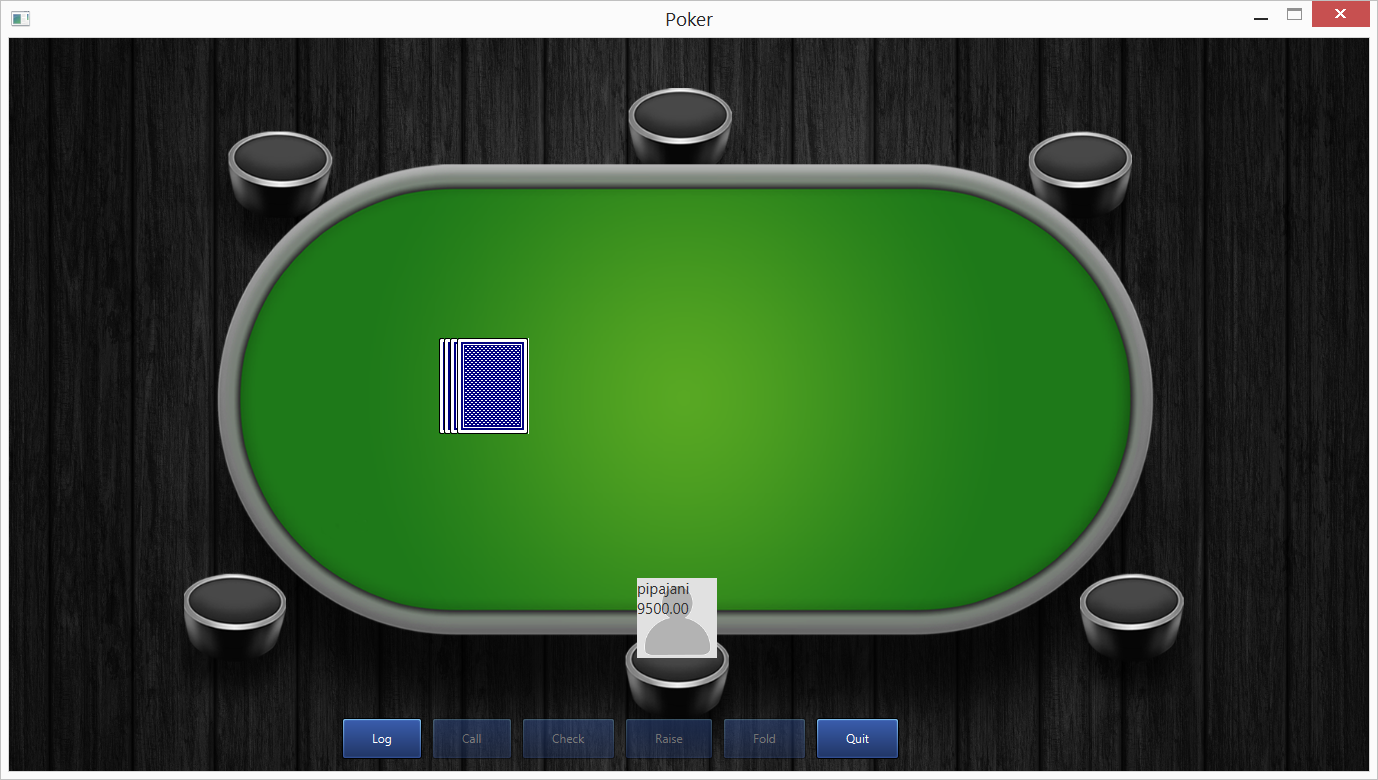
\includegraphics[width=\linewidth]{user-documentation/images/parti/parti_1.jpg}
\end{figure}
A program átirányított minket a \ref{fig:parti_1}. ábrán jelölt felületre. Az üres játékasztal két dolgot jelenthet, vagy azt, hogy az asztalnál éppen játszanak, vagy pedig azt, hogy az asztalnál mi vagyunk az egyedüli játékosok, jelen esetben egyedüliként ülünk az asztalnál. Indítsunk el egy második kliens programot is, majd a fenti utasításokat követve csatlakozzunk az előbbi játék asztalhoz. Miután csatlakoztunk, azután indítsunk el még további három darab kliens programot és csatlakozzunk az előbbi játék asztalhoz. A \ref{fig:sv_log}. árbán láthatjuk a szerver naplózását, amelyről leolvasható, hogy az imént csatlakozott három darab felhasználó várólistára került. \\
\begin{figure}[h!]
  \caption{Szerver naplózása}
  \label{fig:sv_log}
  \centering
    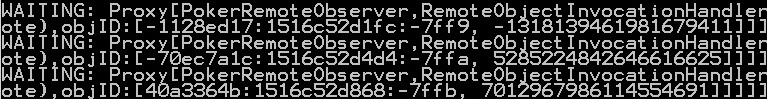
\includegraphics[width=\linewidth]{user-documentation/images/sv_log.jpg}
\end{figure}

Térjünk vissza a játékban lévő kliens programokhoz és játszuk le a megkezdett partit. A következő parti elindulásakor a várólistán szereplő kliensek teljesértékű játékosként csatlakoznak be az éppen elindult partiba, így az asztalnál a \ref{fig:parti_2}. ábra alapján már öt darab játékos fog ülni.
 \begin{figure}[h!]
  \caption{Parti kezdete}
  \label{fig:parti_2}
  \centering
    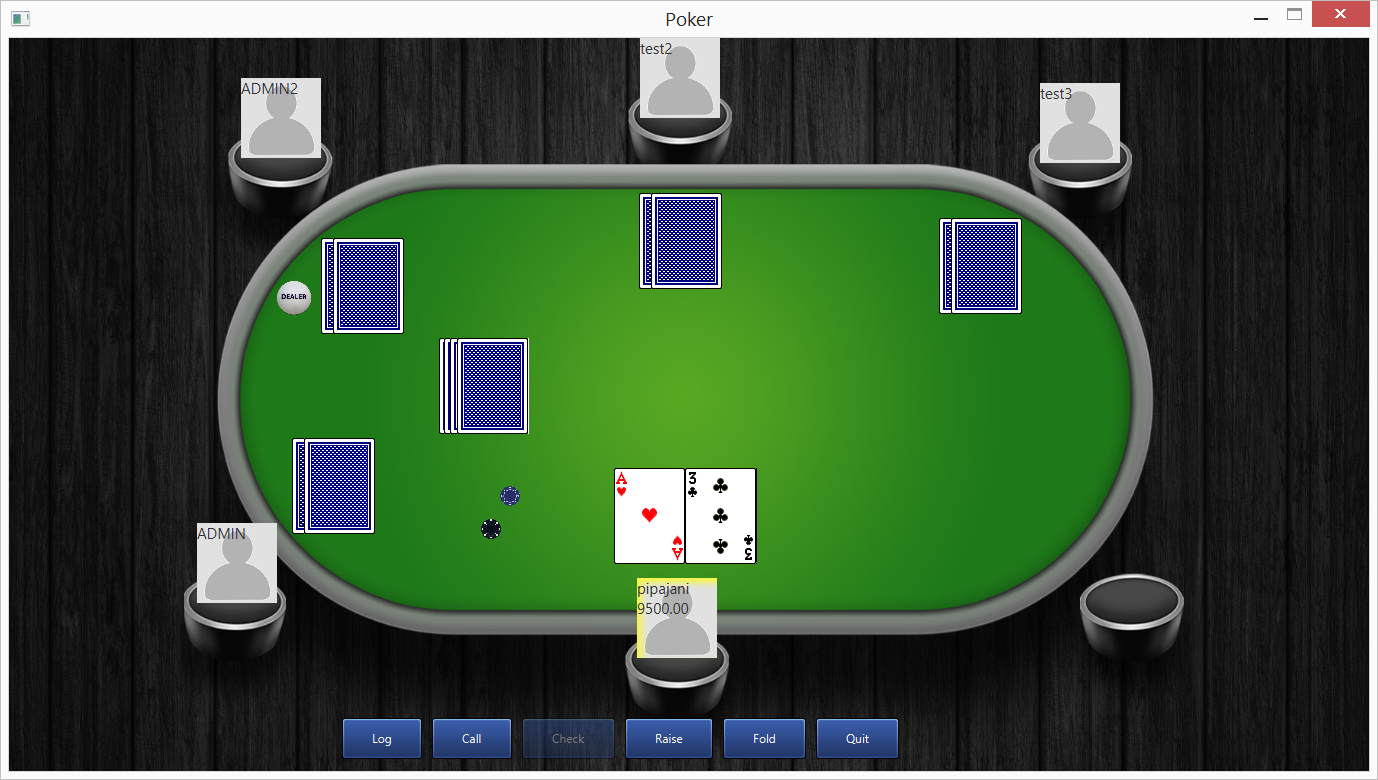
\includegraphics[width=\linewidth]{user-documentation/images/parti/parti_2.jpg}
\end{figure}
Az asztal Texas Hold'Em játékstílusú, így mindenki kettő darab kártyalapot kap kézbe. A kis és nagy vakokat az asztal bekérte, a beadott zsetonok meg is jelentek az asztalon. Jelenleg \texttt{pipajani} következik. Az \texttt{ADMIN2} nevű játékosnál van az osztógomb, tehát a \texttt{test2} nevű játékos a kis és a \texttt{test3} nevű játékos pedig a nagy vak. \texttt{Pipajaninak} az asztal felé nagy vaknyi tartozása van, amelyet az egyenlege alapján meg tud adni. \\
A \ref{fig:parti_3}. ábrán látható, hogy a szerver már kiosztotta mind az öt darab közös lapot és a még senki sem dobta el a lapjait.
 \begin{figure}[h!]
  \caption{RIVER}
  \label{fig:parti_3}
  \centering
    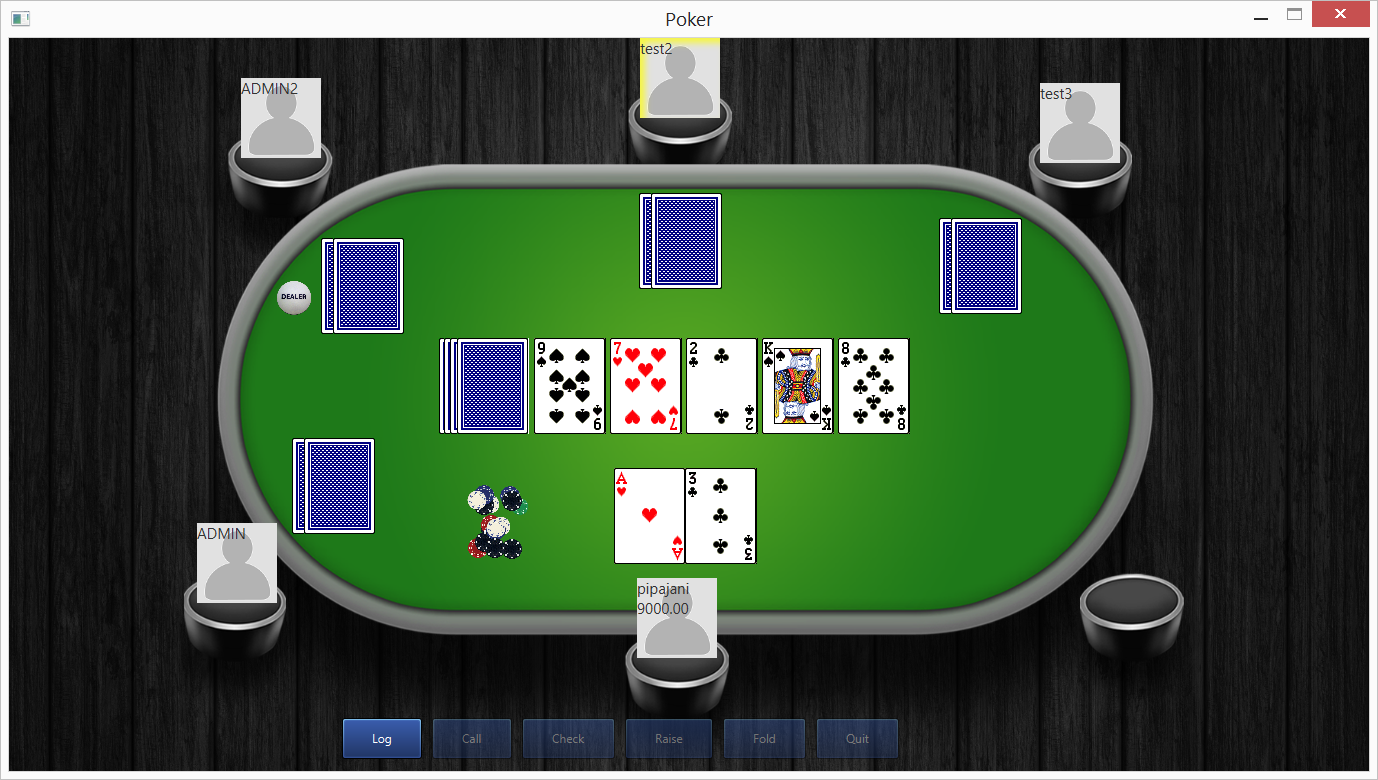
\includegraphics[width=\linewidth]{user-documentation/images/parti/parti_3.jpg}
\end{figure}
A \ref{fig:parti_4}. ábrán már az látható, amikor a parti hamarosan véget ér. A szerver ebben a körben hirdette ki a nyertes lapokat a játékosok között. A \texttt{test3} nevű játékos eldobta a lapjait, azonban értelemszerűen ő is láthatja a nyertes lapokat. Jelenleg a nyertes \texttt{test2} nevű játékos következik. Ha az asztalnál ülő partiban maradt játékosok mindegyikre megnyomta a \texttt{Check} feliratú gombot, akkor a játékasztalon új parti kezdődik. A várakozólistán szereplő játékosok teljes értékű játékosként szerepelnek az asztalnál, továbbá azok a játékosok is kapnak kártyalapokat, akik az előző partiban eldobták a lapjaikat.
 \begin{figure}[h!]
  \caption{Nyertes lapok kihirdetése}
  \label{fig:parti_4}
  \centering
    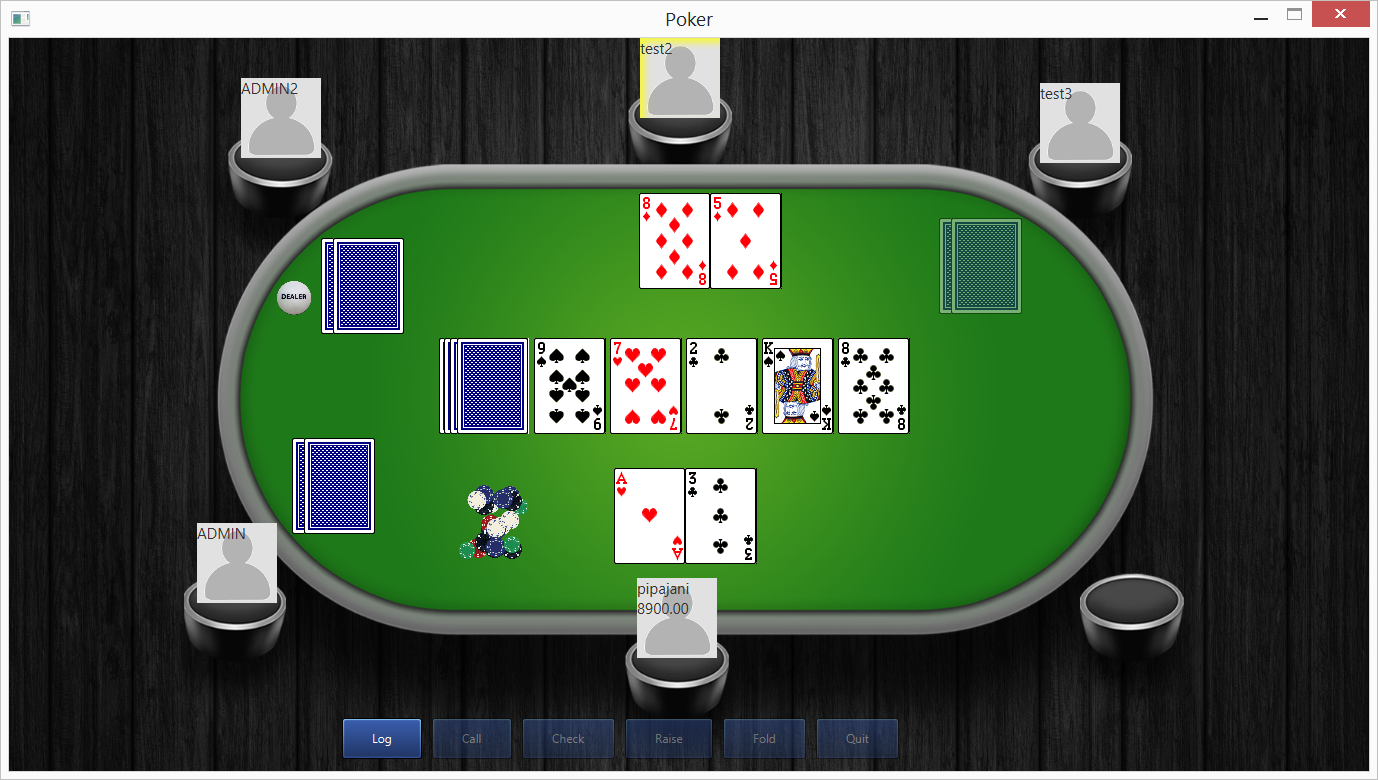
\includegraphics[width=\linewidth]{user-documentation/images/parti/parti_4.jpg}
\end{figure}

\clearpage
